\chapter{Einleitung: Erkenntnisprozess}
\index{Erkenntnisprozess}

In den Naturwissenschaften verl"auft der Erkenntnisprozess im
Allgemeinen "uber die folgenden Stufen:

\begin{description}[\setlabelstyle{\bfseries\slshape}]
\item[Experiment] Von Beobachtungen werden Gesetzm"a"sigkeiten
   abgeleitet
\item[Induktion] Von den Spezellen Gesetzm"a"sigkeiten schlie"st man auf
   allgemeinere Zusammenh"ange
\item[Formulierung] Die allgemeinen Zusammenh"ange werden in einer
   Formel oder als Gesetz \emph{formuliert}
\item[Deduktion] Von Allgemeinen Fall wird auf einen speziellen
   geschlossen und dieser Spezielle durch ein weiteres Experiment
   \emph{verifiziert} oder \emph{falsifiziert}.
\end{description}

Physik ist so \emph{meistens} vorhersagbar -- es gibt aber auch
Gegenbeispiele, bei denen die \emph{Wahrscheinlichkeit} eine wichtige
Rolle spielt.

\begin{Beispiel}
Hier ein paar Beispiele für solch \emph{chaotische} Prozesse.
 \begin{itemize}
\item Wettervorhersage
\item \emph{chaotisches Pendel}
\item \emph{Galton-Brett}
% \begin{figure}
% 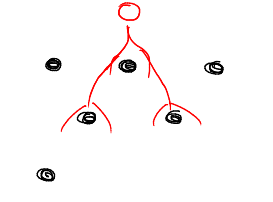
\includegraphics{bilder/fig1}
% \end{figure}
\item \emph{Brownsche Bewegung}

% \begin{figure}[h]
% 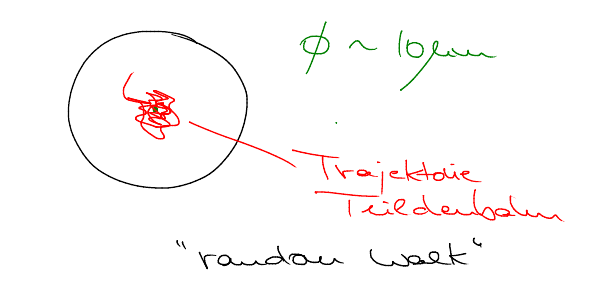
\includegraphics[scale=0.5]{bilder/fig2.png}
% \end{figure}

\item \emph{Quantenmechanik}\\
Es gilt die Heisenbergsche Unschärferelation:
\[
\underbrace{\Delta x}_{\text{Ortsunschärfe}} \cdot \underbrace{\Delta p}_{\text{Impulsunschärfe}}
\]
% \begin{figure}[h]
% 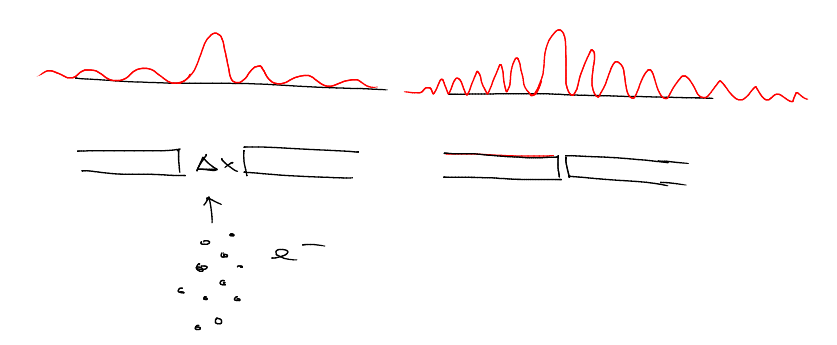
\includegraphics[scale=0.5]{bilder/fig3.png}
% \end{figure}
\end{itemize}
\end{Beispiel}
















